The synthetic nervous system controller is developed with a <insert name here>
neuron model. The neurons are modeled with a resting potential of -60 mV and a
maximum potential of -40 mV for a range of 20 mV.

% TODO(buckbaskin): make the capitalization of the networks consistent

\bbs{Key Neurons and Synapses}

The neuron controller network is made up of a set of engineered synapses
designed to emulate arithmetic operations. These can be grouped into two
categories: excitatory neurons and inhibitory neurons. 

Most neurons were tuned
via an optimization process to identify the best equilibrium potential and
synaptic conductance based on equations defined in 
\cite{NickFunctionalSubnetwork}. 
Some neurons were tuned by hand for specific behaviors in
a subsection of the overall controller.

\bbss{Excitatory Synapses}

Except where otherwise noted, a value of 134 mV was used for the equilibrium
potential. The pre-synaptic threshold is -60 mV and the pre-synaptic saturation
level is -40 mV.

\bbsss{Signal Transfer}

The signal transfer synapse is designed to pass the voltage of the input neuron
to the output neuron in the active range of the neuron. It is often used to add
the value of two or more neurons together in an output neuron.
It has a synaptic 
conductance of 0.115 microsiemens. 

\bbsss{Inverted Signal Transfer}

By combining two signal inversions, a more accurate signal transfer synapse was
created. This involves an extra neuron; however, it leads to a more precise
transfer of the voltage level of the input neuron to the output neuron. In
general, the synapse was implemented with two Signal Inverter (Stimulated)
synapses.

\bbsss{Signal Amplifier 2x}

The signal amplifier synapse is designed to pass the voltage of the input neuron
to the output neuron with a 2x gain. This was tuned with input values from 0 to
10 mV. Higher inputs saturate the output neuron. It has a synaptic conductance
of 0.23 microsiemens.

\bbsss{Signal Amplifier 4x}

The signal amplifier has the same function as the 2x amplifier but with a x4 
gain. This was tuned with input values from 0 to
5 mV. Higher inputs saturate the output neuron. It has a synaptic conductance
of 0.46 microsiemens.

\bbsss{Signal Reduction 0.2x}

The signal reduction synapse is designed to pass the voltage of the input neuron
to the output neuron in the active range of the neuron, but with a loss of 0.2x. 
It has a synaptic  conductance of 0.021 microsiemens. This neuron was tuned
over the complete range of input values, 0 to 20 mV.

\bbsss{Signal Reduction 0.5x}

The signal reduction synapse is designed to pass the voltage of the input neuron
to the output neuron in the active range of the neuron, but with a loss of 0.5x. 
It has a synaptic  conductance of 0.054 microsiemens. This neuron was tuned
over the complete range of input values, 0 to 20 mV.

\bbsss{Convert Forward Positive}

The convert forward positive synapse is designed to convert the representation
of a value in a single neuron, for example the neuron that represents the 
position of the joint, to the same value represented in two neurons. This
synapse converts the value when the value is above -50 mV to values between 0 
and 20 mV. The pre-synaptic
threshold is -50 mV and the synaptic conductance is 0.115 microsiemens.

\bbsss{Torque Pressure Converter}

The torque pressure converter synapse is designed to perform the torque-pressure
calculation approximation. It has a synaptic 
conductance of 0.048 microsiemens.

\bbss{Inhibitory Synapses}

Except where otherwise noted, the equilibrium potential of inhibitory neurons
is simulated as -100 mV. This is the lowest value possible in the simulation.
The pre-synaptic threshold is -60 mV. The pre-synaptic saturation level is -40
mV.

\bbsss{Signal Inverter}

The signal inverted synapse is designed to decrease the voltage of the output 
neuron proportional to the voltage of the input neuron. It has a synaptic 
conductance of 0.55 microsiemens.

\bbsss{Signal Inverter (Stimulated)}

The signal inverted synapse is designed to decrease the voltage of the output 
neuron proportional to the voltage of the input neuron. This synapse is tuned
slightly differently from the standard signal inverter because there was an
observed difference in voltage when a stimulus current was applied to the output
neuron along with other incoming synapses. It has a synaptic 
conductance of 0.5 microsiemens.

\bbsss{Signal Invert Reduction 0.2x}

The signal inverted reduction synapse is designed to decrease the voltage of
the output 
neuron at a 0.2x loss compared to the voltage of the input neuron. It has a 
synaptic conductance of 0.093 microsiemens.

\bbsss{Signal Invert Reduction 0.5x}

The signal inverted reduction synapse is designed to decrease the voltage of
the output 
neuron at a 0.5x loss compared to the voltage of the input neuron. It has a 
synaptic conductance of 0.22 microsiemens.

\bbsss{Signal Inverter Amplifier 2x}

The signal inverted amplifier synapse is designed to decrease the voltage of
the output 
neuron at a 2x gain to the voltage of the input neuron. It has a synaptic 
conductance of 1.11 microsiemens.

\bbsss{Signal Inverter Amplifier 4x}

The signal inverted amplifier synapse is designed to decrease the voltage of
the output 
neuron at a 4x gain to the voltage of the input neuron. It has a synaptic 
conductance of 2.3 microsiemens.

\bbsss{Integral Inhibitor}

The integral inhibitor synapse is designed to help both neurons maintain a 
stable value unless an external current is applied. The values for this
synapse are based on \cite{NickFunctionalSubnetwork}. The synapse has a  
conductance of 0.5 microsiemens.

\bbsss{Convert Forward Negative}

The convert forward negative synapse is designed to convert the representation
of a value in a single neuron, for example the neuron that represents the 
position of the joint, to the same value represented in two neurons. This
synapse converts the value when the value is below -50 mV to a positive value 
from 0 to 20 mV. The pre-synaptic
saturation is -50 mV and the synaptic conductance is 0.5 microsiemens.

\bbsss{Signal Divider}

The signal divider synapse is designed to reduce the effect of another input
synapse, where the reduction increases with increased input voltage to the
signal divider synapse. It is distinguished from the signal multiplier synapse
in that the value never reaches 0. Intuitively, this is a replication of 
division where dividing by a large number makes the quantity small but never 0.
It has a synaptic conductance of 20 microsiemens. The equilibrium potential of
the synapse is -60 mV (equal to the resting potential of the input and output
neurons).

\bbsss{Signal Multiplier}

The signal divider synapse is designed to reduce the effect of another input
synapse, where the reduction decreases with increased input voltage to the
signal divider synapse. It is distinguished from the signal divider synapse
behavior in that the value reaches 0. Intuitively, this is a replication of 
multiplication where multiplying by 0 will make any value 0.
It has a synaptic conductance of 19.75 microsiemens. The equilibrium potential 
of the synapse is -61 mV.

\bbs{Sensor Fusion}

The Sensor Fusion neuron network performs essentially the same function as the
sensor fusion network in the prototype controller. In this case, 3 neurons
represent the 3 sensor inputs available in a joint: position (``Theta"),
extension muscle pressure (``Ext Pres") and flexion muscle pressure
(``Flx Pres"). The outputs for the network are the estimates for current 
position, velocity and acceleration.

\bbss{Velocity Fusion Network Components}

\bbsss{Differentiator Network}

The velocity network is based on the Differentiator Network presented in 
\cite{NickFunctionalSubnetwork}. The key insight into making a network
of neurons that can estimate the derivative of an input signal is that
the time constants of individual neurons can be independently tuned to 
approximate a single step finite difference method. This itself is based
on a Reichardt detector network as explained in
\cite{NickFunctionalSubnetwork}.

% TODO(buckbaskin): Figure of differentiator network

\bbss{Velocity Fusion Network}

The velocity network is based on the Differentiator network. 
The one major change from the network,
as presented, is the inclusion of a second $U_{post}$ neuron to 
represent the negative derivative of the position (negative velocity).

% TODO(buckbaskin): Figure of my velocity network

% TODO(buckbaskin): make sure my inhibitory and excitatory synapses are visualized properly

This represents
a common pattern used across the network where two neurons are used to represent
a single value. One neuron represents positive levels of the variable and is 
at or below resting potential when the value is negative. The other neuron is
above resting potential for negative values and is at or below resting potential
when the value is positive. 

The motivation for increasing the complexity of the
network (often making it more than twice as complicated) is to increase the
effective range of values that the neuron can represent at the same fidelity and
to increase the accuracy of zero. When a single neuron represents positive and
negative values of equal magnitude, the value of 0 is represented at 50 mV; 
however, after passing through a signal transfer synapse this value is often
slightly higher, up to 52 mV. This means that comparing the two neurons (the
original neuron and the signal transfer) yields a slightly positive error
instead of near zero error.

\bbss{Acceleration Fusion Network Components}

\bbsss{Absolute Value Network}

Within the acceleration fusion network, the absolute value of the position is
used. This is calculated by first splitting the position into its two neuron
representation. From there, the sum of the two neurons is used as the absolute
value. This takes advantage of the definition of each side of the two neuron
representation falling below resting potential when the other neuron is active.
This means the signal transfer synapse from the below zero neuron will have no
effect.

% TODO(buckbaskin): Figure of my absolute value network

\bbsss{Integration Network}

The integration network used throughout the neuron controller is based heavily
on the Integrator Network in \cite{NickFunctionalSubnetwork}. Two neurons are
designed to mutually inhibit each other so that the combined pair hold their
values. Individual neurons can be treated as a leaky integrator; however, their
voltage tails off over time if there is no maintenance current. The integration
network itself is tuned by changing the time constant of the component neurons
to adjust how much the voltage of the integrator network changes for an input
current.

\bbsss{Convert Torque to Pressure}

One of the key observations for converting from desired torque to pressure 
within the neuron controller was a pattern observed during simulation. For the
simulated joint, the maximum torque can be applied at an angle of 0 degrees.

\begin{figure}[h!]
\centering
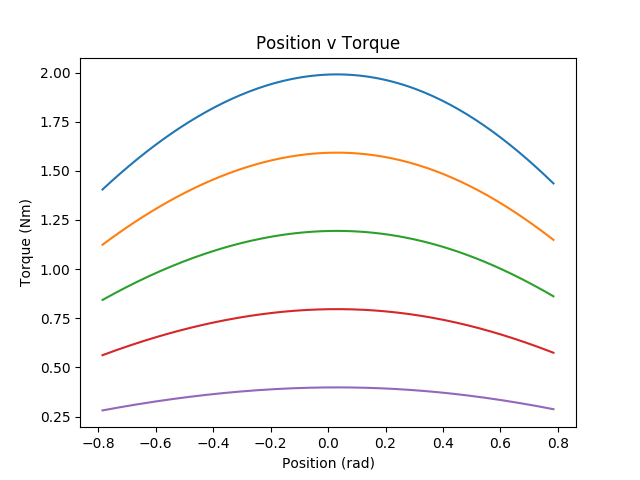
\includegraphics[width=5in]{neuron_design/Pos_v_Torque2.png}
\caption{Position/Torque relation for pneumatic muscle actuated joint}
\label{fig:PositionTorque}
\end{figure}

With increasing deflection, there is decreasing torque applied for a given
pressure, or phrased another way, a greater pressure differential is required
for the same desired torque. When the calculation is rearranged to calculate
a control pressure from a desired torque at a given position, the relationship
between the two is linear for that position for most desired torques above
0.25 Nm in the simulated joint. Assuming there is some non-zero antagonistic
torque, each actuator should fall into the near-linear range. This allows for
an approximation of the linear section in the neuron model.

% TODO(buckbaskin): regenerate the PressureTorque figure with axis labels
\begin{figure}[h!]
\centering
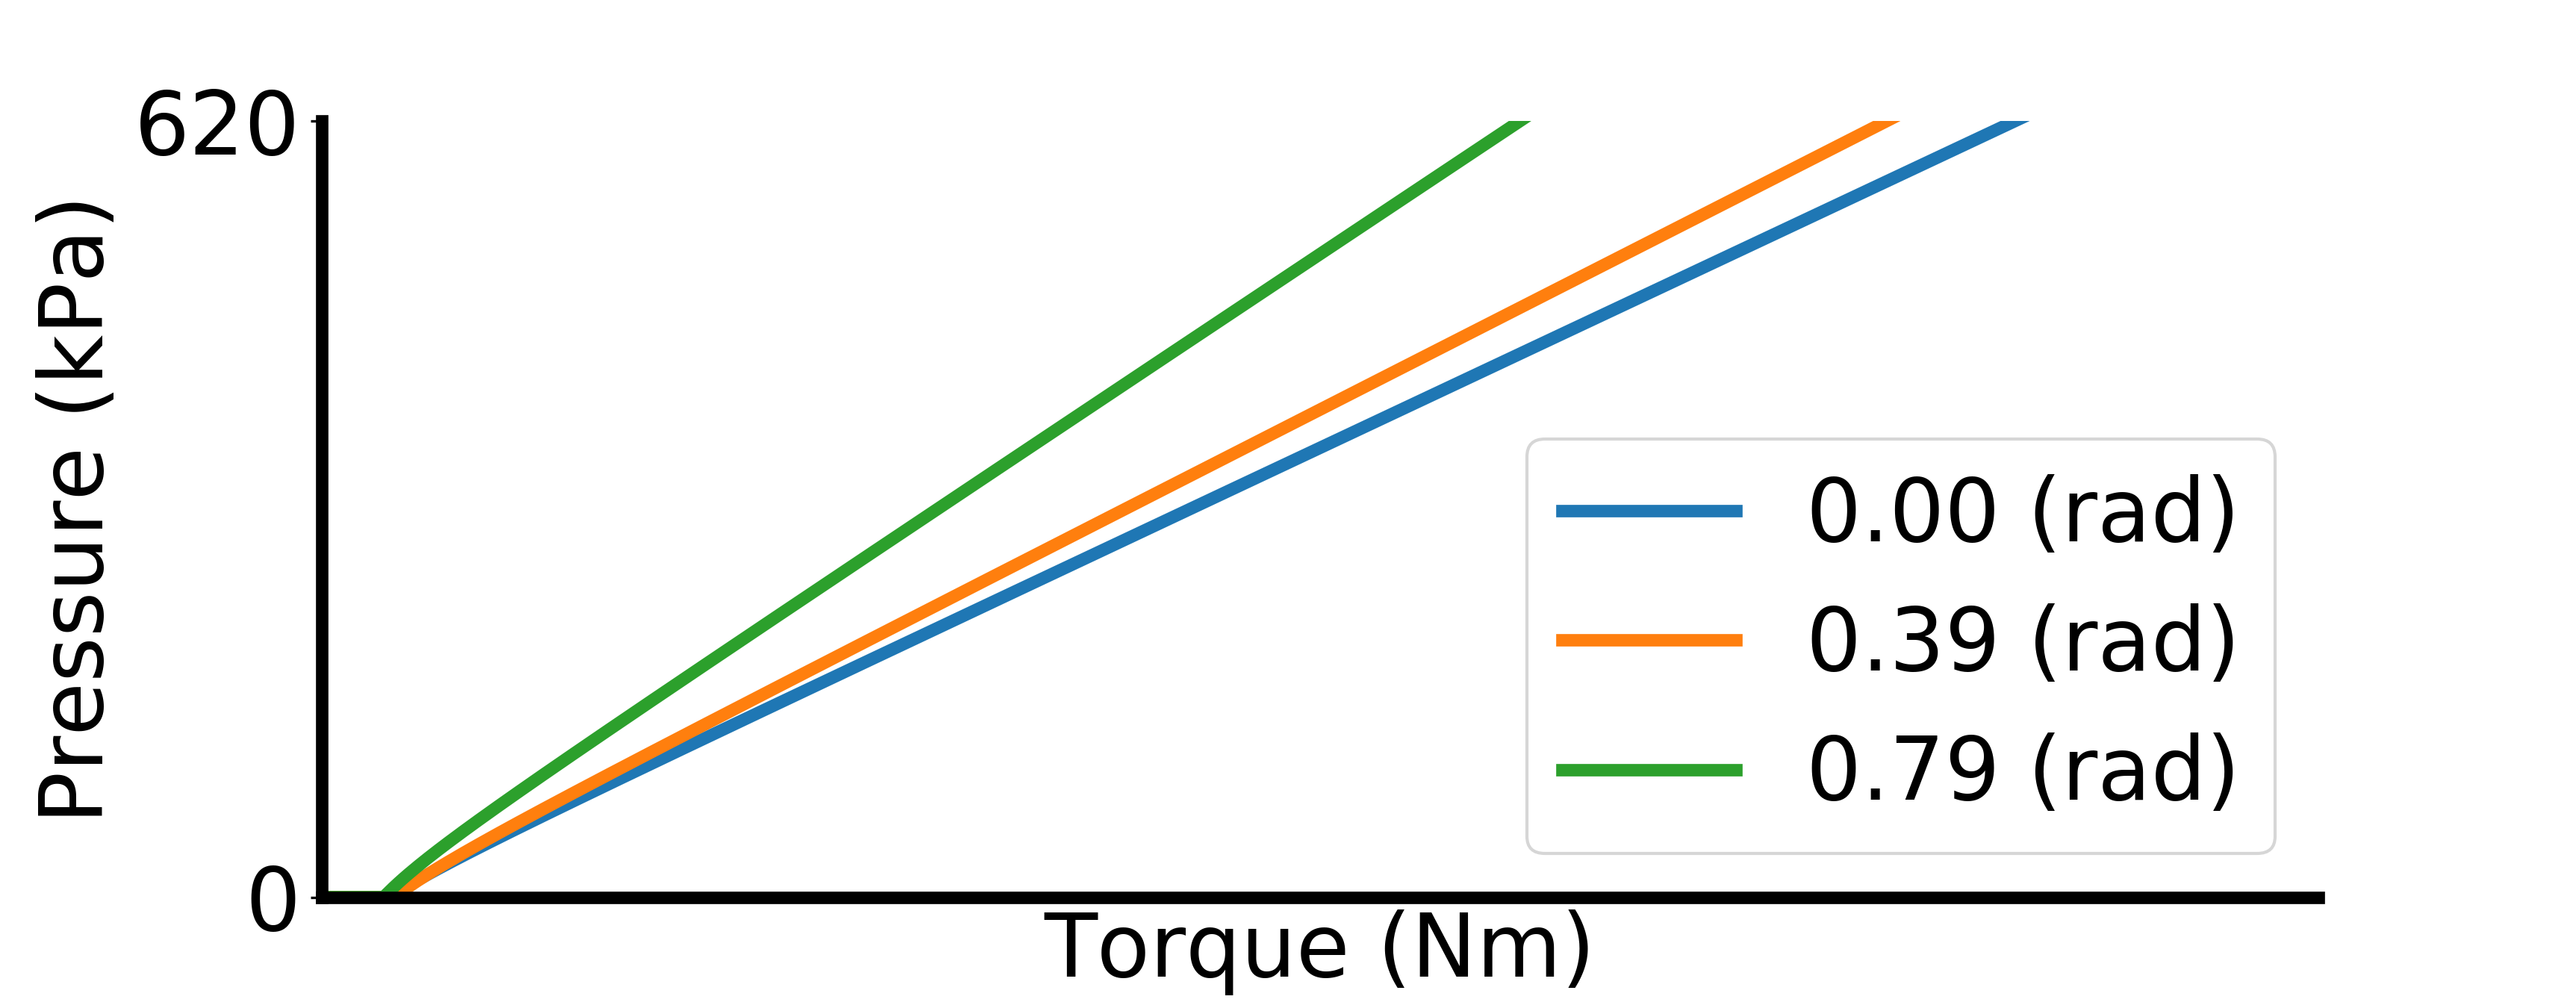
\includegraphics[width=5in]{neuron_design/FigPressureTorque}
\caption{Torque/Pressure relation observed in simulation}
\label{fig:PressureTorque}
\end{figure}

The neurons approximate this relationship using a multiplication synapse added
to a signal transfer synapse. The multiplication takes the scaled absolute 
value of the position as input, so that as the position of the joint reaches
the joint limit, the slope of the torque to pressure curve increases. This
approximates the observations in simulation with a relatively simple neuron
network.

% TODO(buckbaskin): Figure of T2P approximation network

\bbsss{Pressure Estimation Loop}

Within the Acceleration Network, there is a feedback loop that is used to 
estimate the torque applied by a given pressure. First, the loop ``initializes"
with an extension torque guess from the integrator. Second, the extension
torque is converted into extension pressure. Third, the estimated extension
pressure is compared with the sensed pressure. If there is an delta between the
two, the extension torque guess is modified in turn and the cycle repeats.

% TODO(buckbaskin): Figure of pressure loops

This architecture is mirrored for flexion torque.

\bbsss{Torque to Acceleration Network}

The torque to acceleration network is built up in 3 stages. First, a damping 
term is subtracted or added based on the current velocity and the estimated
damping factor. Second, the conservative load is applied to the joint. Third,
the acceleration is attenuated proportional to the mass with a signal divider
synapse.

% TODO(buckbaskin): Figure for T2A

The scaling of the damping factor is the most complicated component of this
network. First, the estimated damping factor is scaled based on the velocity 
with a multiplication synapse to ensure that it has no effect on acceleration
when the velocity is zero. Second, it is then applied with both positive and
negative velocities (in a split representation) to the positive and negative
acceleration terms. Due to the design choice of representing the velocity as two
neurons, this means that one term will be 0 and the other will either have a 
non-zero effect. In code, this would be done as an if statement. In neurons,
all the values and effects are calculated in practice, but only some are passed
through the network.

% TODO(buckbaskin): check and see how the conservative force is applied...

\bbss{Acceleration Fusion Network}

The acceleration fusion network is a combination of an integrator, absolute
value network, the pressure estimation loop and a torque to acceleration
network. In total, the network uses a combination of smaller networks to
estimate the torque applied from sensed pressure and then combine the extension
and flexion torques together to get a net torque and acceleration.

\bbs{Optimizing Torque Control}

The torque control network uses a feedback loop to optimize the
control torque. The network takes the estimated position and velocity from the 
sensor fusion network and the desired position from a trajectory generator
network (ex. a CPG) and outputs the torque to best follow that trajectory.

\bbss{Optimizing Torque Control Components}

\bbsss{Torque Estimation}

The first step in the torque control network is a torque estimate. This is built
as an integration network.

\bbsss{Torque to Acceleration}

This torque to acceleration network is calculated in the same manner as above.
The principle difference is that the source of torque is an desired control
torque instead of the estimated applied torque of the actuators.

\bbsss{Velocity Modification}

% TODO(buckbaskin): Figure - velocity modification network

The velocity modification network takes the current velocity in and adjusts for
the acceleration. Based on the estimated update rate of the controller, the
change in velocity is linear in acceleration.

\begin{equation}
\dot{\theta}_{future} = \dot{\theta}_{current} + \ddot{\theta} * \delta t
\end{equation}

This is encoded as a constant gain (calculated to be 0.2x) to be incorporated 
into to the velocity voltages.

\bbsss{Position Modification}

The position modification network takes the modified velocity in and adjusts the
future position for a time step in the same method as the velocity modification
network.

\begin{equation}
\theta_{future} = \theta_{current} + \dot{\theta}_{future} * \delta t
\end{equation}


\bbsss{Position Comparator}

% TODO(buckbaskin): Figure - position comparator network

The position comparator estimates the error between where the joint will be at
the future point and time and where the trajectory generator wants the joint
to be. This error is used as feedback to directly modify the torque estimate.
This network geometry allows for easy incorporation of other metrics as well.
For example, if the position estimation is noisy, multiple forward projections
can be made for upper and lower bounds and the torque can be optimized to 
minimize an error function over all projected locations.

\bbss{Torque Control Network}

The overall feedback loop and torque control network is a combination of pieces
that joint together to approximate
Newton's Method for finding the root of the error function.

% TODO(buckbaskin): Figure - torque control network overall

The original 
controller used a bounded bisection method that proved less suited for 
implementation in neurons. The bisection method was originally chosen because
it would always converge or have a well defined behavior when the desired
position fell outside the bounds.

\begin{equation}
\theta_{future} = \theta_{current} + (\dot{\theta}_{current} + \ddot{\theta} * \delta t) * \delta t
\end{equation}

\begin{equation}
\theta_{future} = \theta_{current} + \dot{\theta}_{current} * \delta t + \ddot{\theta} * \delta t^{2}
\end{equation}

\begin{equation}
\dfrac{\partial \theta_{future}}{\partial \ddot{\theta}} = \delta t^{2}
\end{equation}

The derivative of the position is constant with respect to the controlled value
$\ddot{\theta}$. Therefore, Newton's Method should also always converges.
Therefore it is a suitable replacement for the bisection method in this neuron
controller. In practice, it should work well with many error functions; however,
a more complicated error function involving multiple independent error 
components may exhibit local minima and a more complex root finding feedback
method may be required.

\bbs{Torque to Pressure}

The torque to pressure section of the network is smaller than the rest of the 
major components. It is built in the same way as the torque to pressure inside
the sensor fusion pressure to torque network. In the sensor fusion application,
the network is used in a forward capacity inside of a feedback loop that ends
up performing an inverse. This network is much more simple because the network
is used only in a forward capacity to compute the desired pressures.

One additional modification to the network is the inclusion of a stiffness
parameter neuron. This controls any desired overlap in the antagonistic control
to increase or decrease joint stiffness manually.

\bbs{System Modeling}

The system modeling network compares the predicted location of the joint from 
the last control iteration with the current position. Using the error 
calculations discussed in \myref{chap:controller_design}, the neuron network
can calculate the weight updates for its internal estimate of damping and 
conservative load. The equations are as follows:

\begin{equation}
\lambda 
=
- \dfrac{2M}{\delta t^{2}} \dfrac{\theta_{err}}{1 + \dot{\theta}_{0}^{2}}
\end{equation}

\begin{equation}
C_{err} = \lambda \dot{\theta}, N_{err} = \lambda
\end{equation}

\bbss{System Modeling Components}

\bbsss{Theta Delay}

The most unique component of the system is the delayed neuron that approximates
the estimated position of the joint. This is done with a signal transfer
synapse and a single neuron with a time constant that is tuned to the controller
update rate.

\bbsss{Prediction Error}

The prediction error is calculated in both a dual neuron representation. The
error is then multiplied with the inertia, again resulting in a dual 
representation of the positive and negative quantity. This matches the behavior
expressed in the first term of the update equation to calculate $\lambda$.

\bbsss{Velocity Correction}

The absolute value of the velocity is used along with a signal divider. This
matches the second term of the equation to calculate $\lambda$. In practice,
the divider network is one of the networks that fits closely to a term like
$\dfrac{1}{1 + x^{2}}$. One potential improvement to the network is to fit
a custom synapse or sub-network to better fit the term; however, this is not
currently a major source of error.

\bbsss{Lambda Calculation}

The calculation of $\lambda$ is completed with the addition of a gain term. This
allows for the scaling of the updates and behaves in a similar way to the 
learning rate in a neural network. A single data point may be noisy, but if a 
series of updates suggest the same parameter update, the network will adjust the
parameter.

\bbsss{Calculating $\Delta N$}

The calculation for the conservative load is simply a signal transfer from the scaled lambda, following the given equation.

\bbsss{Calculating $\Delta C$}

The calculation for the damping factor update is more involved. In particular,
the complexity comes from the fact that the sign of the update changes with the
sign of the velocity and the positional error. Intuitively, this happens because
damping opposes velocity, but conservative loads (as modeled) don't depend on
velocity. For example, a positive velocity and positive $\lambda$ means that 
less actual damping occurred than was expected, but a negative velocity with a 
positive $\lambda$ means that more damping occurred than was expected.

% TODO(buckbaskin): connect up signed velocities to C calculation
% TODO(buckbaskin): chcek the sign of the C update and make sure it matches written text

To perform this calculation in neurons, the velocity and $\lambda$ are 
calculated for all sign pairs. From there, the correct outputs are connected.
Following the example above, a positive velocity and positive $\lambda$ transfer
their signal to the positive C delta, which then connects to the damping factor 
to drive it down. For a positive lambda and a negative velocity, the ``C Err -+" neuron is active and this transfers to the negative C Delta output.

This implementation relies on the dual neuron representation for values to drive
the correct output. Either the positive or negative neuron will be active in the
velocity and $\lambda$ values, therefore only one of the 4 combination neurons
will be active meaning that only the correct sign of the output value will be
active, maintaining the correctness of the dual neuron representation in the 
output. This implementation replaces a series of if statements that may appear
in a code-defined controller and shows an additional advantage of using two
neurons to represent a value in a functional sub-network. When connected 
correctly, it allows for easier sign flipping, easier validation of correctness
by checking edge connectivity and easier testing.

\bbs{Combined Controller Network}

% TODO(buckbaskin): figure out how to reference a figure
% TODO(buckbaskin): I like splitting out subnetwork into sub-network, but idk if it's consistent with Nick's/Alex's work 
The fully combined network (see Figure how do I reference a figure?) implements
a controller by combining the 4 large sub-networks. First, sensor data is passed
through a sensor fusion network. The state estimation output of the sensor 
fusion network are then passed into the torque optimization network. The 
selected torque is then passed through one more sub-network to convert the
desired torque into pressures for the actuators.

\begin{figure}[h!]
\centering
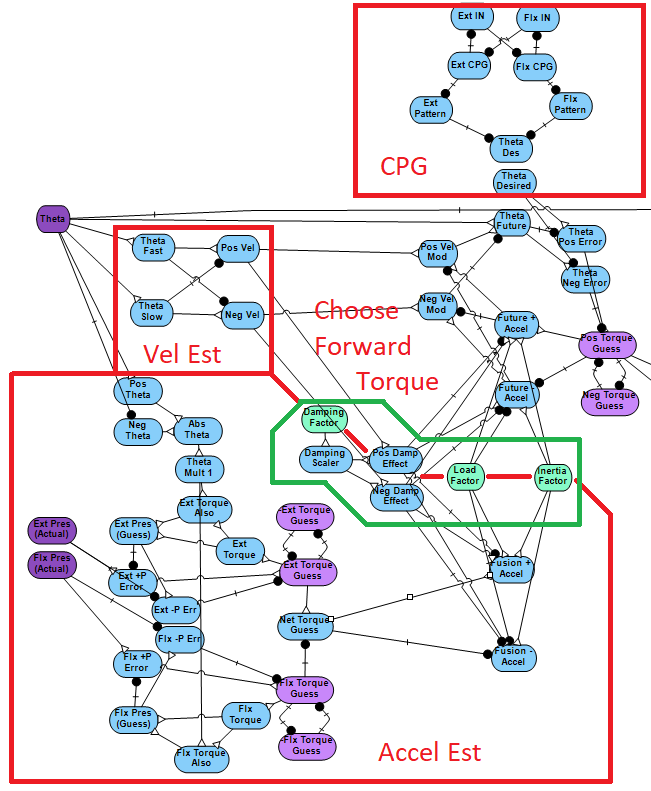
\includegraphics[width=5in]{neuron_design/NetworkLayout}
\caption{Overview of major network components}
\label{fig:NetworkLayout}
\end{figure}
% TODO(buckbaskin): redo this with the complete actual network

This leaves the system model sub-network. This last sub-network is connected to 
the state estimation values and the internal projection and observes the 
differences between the forward prediction and reality. This observer then 
updates key model parameters to improve the controller over time while 
maintaining a controller that avoids excessive oscillation. 
